\documentclass[14pt]{extarticle}

\usepackage{amsmath}
\usepackage{amssymb}
\usepackage{amsthm}
\usepackage[a4paper,margin=2.5cm]{geometry}
\usepackage{xcolor}
\usepackage{graphicx}
\usepackage{enumitem}
\usepackage{titlesec}
\usepackage[most]{tcolorbox}
\usepackage{colortbl}
\usepackage{array}
\usepackage{hyperref}
\hypersetup{colorlinks=true,linkcolor=blue,urlcolor=blue}

\usepackage{xepersian}
\settextfont{Vazirmatn FD}

\setlength{\emergencystretch}{3em}
\hyphenpenalty=10000
\exhyphenpenalty=10000

\definecolor{headblue}{RGB}{200,90,140}
\definecolor{boxbg}{RGB}{252,240,246}
\definecolor{claimbg}{RGB}{250,235,243}
\definecolor{proofaccent}{RGB}{225,180,200}

% ---- section / subsection styling ----
\titleformat{\section}
  {\Large\bfseries\color{headblue}}{\thesection}{0.6em}{}
  [{\vspace{2pt}\color{headblue!35}\titlerule[1.2pt]}]
\titlespacing*{\section}{0pt}{0pt}{12pt}
\titleformat{\subsection}
  {\large\bfseries\color{headblue!88}}{\thesubsection}{0.5em}{}
\titlespacing*{\subsection}{0pt}{10pt}{6pt}

% ---- claim box ----
\newtcolorbox{claimx}{
  breakable, enhanced, boxrule=0pt, arc=3pt,
  colback=claimbg, frame hidden,
  borderline east={3pt}{0pt}{headblue},
  left=10pt, right=12pt, top=7pt, bottom=7pt,
  before upper={\textbf{\color{headblue}ادعا.}\enspace}
}

% ---- proof box ----
\newtcolorbox{proofx}{
  breakable, enhanced, blanker,
  borderline east={2pt}{0pt}{proofaccent},
  left=12pt, right=4pt, top=4pt, bottom=4pt,
  before upper={\textbf{اثبات.}\enspace}
}

\newcommand{\R}{\mathbb{R}}
\newcommand{\norm}[1]{\left\lVert #1 \right\rVert}
\newcommand{\T}{^{\top}}

\begin{document}

\noindent{\small\textbf{ملیکا زارع}\quad\textbar\quad شماره دانشجویی: ۴۰۱۱۳۴۱۶\quad\textbar\quad{\color{black!65} جبر خطی عددی --- تمرین سری چهارم}}
\vspace{4pt}
{\color{headblue!40}\hrule height 1pt}
\vspace{10pt}

%==================================================================
\section{گام ۲ --- ماتریس تشابه: تقارن (پرسش ۱-الف)}
%==================================================================

هر پیکسل را یک گره در نظر می‌گیریم و وزن یالِ میان دو پیکسل $i$ و $j$ را طبق رابطه‌ی (۱) این‌طور تعریف می‌کنیم:
\[
W_{ij}=
\begin{cases}
\exp\!\left(\dfrac{-\norm{F_i-F_j}_2^{2}}{\sigma_I^{2}}\right)\cdot
\exp\!\left(\dfrac{-\norm{X_i-X_j}_2^{2}}{\sigma_X^{2}}\right), & \norm{X_i-X_j}_2 < r,\\[12pt]
0, & \text{در غیر این صورت,}
\end{cases}
\]
و طبق قرارداد $W_{ii}=0$ (هیچ گره ای با خودش یال ندارد).

\begin{claimx}
ماتریس $W$ دقیقاً متقارن است؛ یعنی برای هر زوج پیکسل $i$ و $j$ همواره $W_{ij}=W_{ji}$ برقرار است.
\end{claimx}

\noindent\textbf{بخش (الف): اثبات تحلیلی تقارن ماتریس $W$.}
برای اثبات اینکه ماتریس $W$ دقیقاً متقارن است، باید نشان دهیم که برای هر زوج پیکسل $i$ و $j$، رابطه‌ی $W_{ij}=W_{ji}$ همواره برقرار است. فرمولِ وزن برای حالتِ $\norm{X_i-X_j}_2<r$ به شکلِ زیر است:
\[
W_{ij}=\exp\!\left(-\frac{\norm{F_i-F_j}_2^{2}}{\sigma_I^{2}}\right)\cdot
\exp\!\left(-\frac{\norm{X_i-X_j}_2^{2}}{\sigma_X^{2}}\right).
\]

\begin{proofx}
می‌دانیم که نرم-۲ (فاصله‌ی اقلیدسی) دارای خاصیتِ همگنیِ مطلق است؛ یعنی برای هر بردارِ $V$ و عددِ ثابتِ $c$ داریم $\norm{cV}=|c|\,\norm{V}$. اگر $c=-1$ باشد:
\[
\norm{F_i-F_j}_2=\norm{(-1)(F_j-F_i)}_2=|-1|\cdot\norm{F_j-F_i}_2=\norm{F_j-F_i}_2 .
\]
با به توان رساندنِ طرفین، نتیجه می‌گیریم که فاصله‌ی روشناییِ دو پیکسل از هر طرف که محاسبه شود یکسان است:
\[
\norm{F_i-F_j}_2^{2}=\norm{F_j-F_i}_2^{2} .
\]
\[
\norm{X_i-X_j}_2^{2}=\norm{X_j-X_i}_2^{2} .
\]

شرطِ فاصله‌ی مکانی، یعنی $\norm{X_i-X_j}_2<r$، نیز با توجه به اثباتِ بالا دقیقاً معادلِ شرطِ $\norm{X_j-X_i}_2<r$ است.

اکنون اگر فرمولِ $W_{ji}$ را بنویسیم:
\[
W_{ji}=\exp\!\left(-\frac{\norm{F_j-F_i}_2^{2}}{\sigma_I^{2}}\right)\cdot
\exp\!\left(-\frac{\norm{X_j-X_i}_2^{2}}{\sigma_X^{2}}\right),
\]
با جایگذاریِ تساوی‌های به‌دست‌آمده از گامِ اول، به‌وضوح به معادله‌ی اصلی می‌رسیم:
\[
W_{ji}=\exp\!\left(-\frac{\norm{F_i-F_j}_2^{2}}{\sigma_I^{2}}\right)\cdot
\exp\!\left(-\frac{\norm{X_i-X_j}_2^{2}}{\sigma_X^{2}}\right)=W_{ij}.
\]
چون برای حالتِ $\norm{X_i-X_j}_2\ge r$ نیز مقدارِ هر دو درایه‌ی $W_{ij}$ و $W_{ji}$ برابرِ صفر تعریف شده است، پس در تمامیِ حالات $W_{ij}=W_{ji}$ برقرار بوده و ماتریسِ $W$ ذاتاً یک ماتریسِ متقارن است.
\end{proofx}

\noindent\textbf{تأیید عددی (پرسش ۱-ب).}
در کد مقدارِ $\norm{W-W\T}_F$ را محاسبه کردیم و برابرِ $0$ شد؛ پس تقارن به‌صورتِ عددی هم تأیید می‌شود.

\medskip
\noindent\textbf{مقادیرِ انتخابی.} $\sigma_I=0.1$، $\sigma_X=4$ و $r=5$ (برحسبِ پیکسل). این سه پارامتر تعیین می‌کنند که «شباهت» بینِ دو پیکسل چقدر سخت‌گیرانه سنجیده شود:

\smallskip
\noindent$\bullet$~\textbf{$\sigma_I$} هرچه بزرگ‌تر باشد، اختلافِ روشناییِ بیشتری تحمل می‌شود، وزن‌ها یکنواخت‌تر می‌شوند و مرزها نرم‌تر درمی‌آیند؛ اگر خیلی کوچک باشد فقط پیکسل‌های تقریباً هم‌رنگ به هم وصل می‌مانند و قطعه‌بندی به نویز حساس می‌شود.

\smallskip
\noindent$\bullet$~\textbf{$\sigma_X$} بزرگ‌ترشدنش پیکسل‌های دورتر را هم به هم پیوند می‌دهد و نواحیِ گسترده‌تری می‌سازد؛ کوچک‌بودنش گراف را محلی‌تر و قطعه‌ها را ریزتر می‌کند.

\smallskip
\noindent$\bullet$~\textbf{$r$} شعاعِ همسایگی است؛ یال فقط بین پیکسل‌هایی با فاصله‌ی کمتر از $r$ برقرار می‌شود؛ این برش، ماتریسِ $W$ را \emph{تُنُک} نگه می‌دارد و هزینه‌ی محاسبات را کم می‌کند.

\newpage
%==================================================================
\section{گام ۳ --- لاپلاسین نرمال‌شده (پرسش ۲)}
%==================================================================

درجه‌ی هر گره $d_i=\sum_j W_{ij}$، ماتریس درجه $D=\operatorname{diag}(d_1,\dots,d_n)$، و
\[
L_{\mathrm{sym}}=D^{-1/2}(D-W)D^{-1/2}=I-D^{-1/2}W D^{-1/2}.
\]

%------------------------------------------------------------------
\subsection{الف) تقارن \texorpdfstring{$L_{\mathrm{sym}}$}{Lsym}}
%------------------------------------------------------------------

\begin{proofx}
از فرمِ $L_{\mathrm{sym}}=I-D^{-1/2}W D^{-1/2}$ شروع می‌کنیم و برای گرفتنِ ترانهاده از دو ویژگیِ جبرِ خطی استفاده می‌کنیم: (۱) $(A-B)\T=A\T-B\T$، و (۲) $(ABC)\T=C\T B\T A\T$. بنابراین
\[
L_{\mathrm{sym}}\T=\bigl(I-D^{-1/2}W D^{-1/2}\bigr)\T
= I\T-\bigl(D^{-1/2}W D^{-1/2}\bigr)\T .
\]
\begin{itemize}[leftmargin=1.6em,itemsep=1pt,topsep=2pt]
\item ماتریسِ همانی متقارن است، پس $I\T=I$.
\item چون $D$ قطری است، $D^{-1/2}$ هم قطری و در نتیجه متقارن است: $(D^{-1/2})\T=D^{-1/2}$.
\item در پرسشِ ۱ ثابت کردیم که ماتریسِ مجاورت متقارن است، پس $W\T=W$.
\end{itemize}
\[
\bigl(D^{-1/2}W D^{-1/2}\bigr)\T=(D^{-1/2})\T\,W\T\,(D^{-1/2})\T
= D^{-1/2}W D^{-1/2}.
\]
پس در نهایت
\[
L_{\mathrm{sym}}\T = I-D^{-1/2}W D^{-1/2}=L_{\mathrm{sym}} ,
\]
و به‌صورتِ تحلیلی ثابت شد که $L_{\mathrm{sym}}$ ماتریسی متقارن است.
\end{proofx}

%------------------------------------------------------------------
\subsection{ب) حقیقی بودن طیف و قرارگیری در بازه‌ی \texorpdfstring{$[0,2]$}{[0,2]}}
%------------------------------------------------------------------

\noindent\textbf{تحلیلِ تئوری.}
در بخشِ (الف) ثابت کردیم که $L_{\mathrm{sym}}$ متقارن است. «اگر $A$ ماتریسی حقیقی و متقارن باشد، همه‌ی مقادیر ویژه‌اش حقیقی‌اند.» در نظریه‌ی گرافِ طیفی نشان داده می‌شود که لاپلاسینِ نرمال‌شده \emph{نیمه‌معینِ مثبت} است (یعنی $\lambda_i\ge 0$) و بزرگ‌ترین مقدار ویژه‌اش همواره $\lambda_{\max}\le 2$ است.

\smallskip
\noindent برای اثباتِ دقیقِ بازه، کافی است نشان دهیم هم $L_{\mathrm{sym}}$ و هم $2I-L_{\mathrm{sym}}$
نیمه‌معینِ مثبت‌اند؛ اولی کرانِ پایینِ $0$ و دومی کرانِ بالای $2$ را تضمین می‌کند.

\begin{proofx}
قرار می‌دهیم $y=D^{-1/2}x$. آنگاه
\begin{align*}
x\T L_{\mathrm{sym}}\,x
&= x\T D^{-1/2}(D-W)D^{-1/2}x = y\T(D-W)y\\
&=\tfrac12\sum_{i,j}W_{ij}\,(y_i-y_j)^2\;\ge 0 ,
\end{align*}
این یعنی $L_{\mathrm{sym}}\succeq 0$ و بنابراین همه‌ی مقادیر ویژه $\ge 0$ هستند.
حالا به سراغِ کرانِ بالا می‌رویم:
\[
2I-L_{\mathrm{sym}} = I + D^{-1/2}W D^{-1/2}=D^{-1/2}(D+W)D^{-1/2},
\]
و مشابه بالا
\begin{align*}
x\T(2I-L_{\mathrm{sym}})x
&= y\T(D+W)y=\tfrac12\sum_{i,j}W_{ij}\,(y_i+y_j)^2\;\ge 0 ,
\end{align*}
پس $2I-L_{\mathrm{sym}}\succeq 0$ و همه‌ی مقادیر ویژه $\le 2$ هستند. این دو کران کنارِ هم نشان می‌دهند که کلِ طیف داخلِ $[0,2]$ جا می‌گیرد.
\end{proofx}

\noindent\textbf{تأیید عددی.} در کد طیف را محاسبه کردیم: کوچک‌ترین مقدار ویژه حدودِ $-2\times10^{-15}$
(عملاً صفر) و بزرگ‌ترین حدودِ $1.08$ به دست آمد، که با بازه‌ی $[0,2]$ سازگار است.

%------------------------------------------------------------------
\subsection{ج) کوچک‌ترین مقدار ویژه‌ی صفر و بردار ویژه‌ی بدیهی}
%------------------------------------------------------------------

\begin{claimx}
$\lambda=0$ مقدار ویژه‌ی $L_{\mathrm{sym}}$ است و بردار ویژه‌ی متناظرش
$v_0=D^{1/2}\mathbf{1}=(\sqrt{d_1},\dots,\sqrt{d_n})\T$ است.
\end{claimx}

\begin{proofx}
برای اثباتِ اینکه $v_0=D^{1/2}\mathbf{1}$ بردارِ ویژه با مقدار ویژه‌ی $\lambda=0$ است، باید نشان دهیم $L_{\mathrm{sym}}v_0=0\cdot v_0=\mathbf 0$ (بردارِ $\mathbf 1$ همان برداری است که همه‌ی درایه‌هایش $1$ است). داریم
\begin{align*}
L_{\mathrm{sym}}\,(D^{1/2}\mathbf{1})
&=(I-D^{-1/2}W D^{-1/2})(D^{1/2}\mathbf{1})\\
&=D^{1/2}\mathbf{1}-D^{-1/2}W\,(D^{-1/2}D^{1/2})\mathbf{1}
=D^{1/2}\mathbf{1}-D^{-1/2}(W\mathbf{1}).
\end{align*}
حالا به تعریفِ ماتریسِ درجه دقت کنیم: $d_i=\sum_j W_{ij}$؛ یعنی ضربِ $W$ در بردارِ $\mathbf 1$ (که معادلِ جمع‌زدنِ سطرهای $W$ است) دقیقاً بردارِ درجه‌ها را می‌دهد: $W\mathbf{1}=D\mathbf{1}$. با جایگذاری:
\[
L_{\mathrm{sym}}\,(D^{1/2}\mathbf{1})
=D^{1/2}\mathbf{1}-D^{-1/2}(D\mathbf{1})
=D^{1/2}\mathbf{1}-D^{1/2}\mathbf{1}=\mathbf{0}.
\]
پس $D^{1/2}\mathbf 1$ بردارِ ویژه‌ی متناظر با مقدار ویژه‌ی صفر است؛ و چون از قسمتِ قبل می‌دانیم طیف نامنفی است، همین $\lambda=0$ کوچک‌ترین مقدار ویژه است.
\end{proofx}

\noindent\textbf{چرا این بردار ویژه اطلاعاتی برای قطعه‌بندی ندارد؟}

بردارِ ویژه‌ی متناظر با مقدار ویژه‌ی صفر، حالتی را نشان می‌دهد که کلِ گراف (تصویر) به‌عنوانِ یک «مجموعه‌ی واحد و پیوسته» در نظر گرفته شده و هیچ برشی در آن رخ نداده است. چون همه‌ی درایه‌های این بردار متناسب با ریشه‌ی درجه‌ی گره‌ها ($\sqrt{d_i}$) و همگی هم‌علامت‌اند، نمی‌توانند گره‌ها را به دو یا چند دسته‌ی مجزا تفکیک کنند؛ پس برای عملِ «قطعه‌بندی» که نیازمندِ جداسازی است بی‌فایده‌اند و کنار گذاشته می‌شوند.

%------------------------------------------------------------------
\subsection{د) ارتباط با کیفیت «برش» گراف}
%------------------------------------------------------------------

ماتریسِ $L_{\mathrm{sym}}$ شکلِ نرمال‌شده‌ای از ساختارِ گراف است که هم ارتباطاتِ بینِ گره‌ها (از طریقِ $W$) و هم تراکمِ محلیِ هر گره (از طریقِ $D$) را در بر می‌گیرد و برای حلِ تقریبیِ مسئله‌ی بهینه‌سازیِ «برشِ نرمال‌شده» ساخته می‌شود. فرمِ درجه‌دومش
$x\T L_{\mathrm{sym}}x=\tfrac12\sum_{ij}W_{ij}(y_i-y_j)^2$ (با $y=D^{-1/2}x$) هزینه‌ی برشِ گراف را اندازه می‌گیرد؛ اگر دو پیکسلِ شبیه و نزدیک برچسبِ متفاوت بگیرند جریمه می‌شویم. مقادیر ویژه‌ی کوچکِ این ماتریس نشان‌دهنده‌ی برش‌هایی‌اند که کمترین هزینه (وزنِ یال‌های قطع‌شده) را نسبت به حجمِ نواحیِ جداشده دارند؛ به همین دلیل بردارهای ویژه‌ی متناظر با کوچک‌ترین مقادیر ویژه‌ی ناصفر، بهترین توابعِ نشانگر برای تفکیکِ گراف به نواحیِ متراکم و معنادار با مرزهای ضعیف (قطعه‌بندیِ بهینه) محسوب می‌شوند.

\newpage
%==================================================================
\section{گام ۴ --- روش حذف (پرسش ۳)}
%==================================================================

فرض کنیم $A$ یک ماتریسِ متقارنِ حقیقیِ $n\times n$ باشد با مقادیر ویژه‌ی
$\lambda_1,\dots,\lambda_n$ و بردارهای ویژه‌ی \emph{یکه و دوبه‌دو متعامدِ}
$X_1,\dots,X_n$؛ یعنی $X_1\T X_1=1$ و برای $i\neq j$ داریم $X_j\T X_i=0$، و معادله‌ی مقدار ویژه $A X_i=\lambda_i X_i$ برقرار است. ماتریسِ حذف‌شده را این‌طور می‌سازیم:
\[
B = A - \lambda_1 X_1 X_1\T .
\]

\begin{claimx}
بردارهای ویژه‌ی $B$ دقیقاً همان بردارهای ویژه‌ی $A$ هستند؛ مقدار ویژه‌ی متناظر با $X_1$
به صفر تبدیل می‌شود و سایر مقادیر ویژه بدون تغییر می‌مانند.
\end{claimx}

\begin{proofx}
اثرِ $B$ را روی $X_1$ و روی سایرِ بردارها جداگانه بررسی می‌کنیم.

\textbf{بخشِ اول --- اثرِ $B$ روی $X_1$:} با پخش‌کردنِ $X_1$ در پرانتز داریم
\[
B X_1 = (A-\lambda_1 X_1 X_1\T)X_1 = A X_1 - \lambda_1 X_1 (X_1\T X_1).
\]
طبقِ فرض $A X_1=\lambda_1 X_1$، و چون $X_1$ یکه است $X_1\T X_1=1$؛ پس
\[
B X_1 = \lambda_1 X_1 - \lambda_1 X_1\cdot 1 = \mathbf{0}=0\cdot X_1 .
\]
یعنی $X_1$ همچنان بردارِ ویژه‌ی $B$ است، اما با مقدار ویژه‌ی $0$؛ پس $\lambda_1$ حذف شده است.

\textbf{بخشِ دوم --- اثرِ $B$ روی $X_i$ برای $i\neq 1$:} این‌بار چون بردارهای ویژه‌ی ماتریسِ متقارن متعامدند، $X_1\T X_i=0$؛ پس
\[
B X_i = A X_i - \lambda_1 X_1 (X_1\T X_i) = \lambda_i X_i - \lambda_1 X_1\cdot 0 = \lambda_i X_i .
\]
یعنی $X_i$ دست‌نخورده می‌ماند و همان مقدار ویژه‌ی $\lambda_i$ را حفظ می‌کند.

نتیجه اینکه $B$ همان بردارهای ویژه‌ی $A$ را دارد و فقط طیفش به
$\{0,\lambda_2,\lambda_3,\dots,\lambda_n\}$ تغییر کرده است. بنابراین اگر پیش‌تر $|\lambda_1|$ غالب بود،
اکنون $\lambda_2$ مقدار ویژه‌ی غالبِ $B$ است و می‌توان روشِ تکراری را دوباره روی $B$ اجرا کرد.
\end{proofx}

\newpage
%==================================================================
\section{گام ۴ --- تعامد و تکرار حذف (پرسش ۴)}
%==================================================================

%------------------------------------------------------------------
\subsection{الف) تعامد بردارهای ویژه‌ی ماتریس متقارن}
%------------------------------------------------------------------

\begin{claimx}
اگر $A$ متقارن حقیقی باشد و $X_i,X_j$ بردارهای ویژه‌ی متناظر با مقادیر ویژه‌ی
\emph{متمایز} $\lambda_i\neq\lambda_j$ باشند، آنگاه $X_i\perp X_j$.
\end{claimx}

\begin{proofx}
از معادلاتِ مقدار ویژه شروع می‌کنیم: $A X_i=\lambda_i X_i$ و $A X_j=\lambda_j X_j$. کمیتِ $X_j\T A X_i$ را به دو روش محاسبه می‌کنیم. از یک سو با استفاده از $A X_i=\lambda_i X_i$:
\[
X_j\T A X_i = X_j\T(\lambda_i X_i)=\lambda_i\,(X_j\T X_i).
\]
از سوی دیگر، چون $X_j\T A X_i$ یک اسکالر است، با خودش برابرِ ترانهاده‌اش است، و با به‌کارگیریِ تقارنِ $A\T=A$:
\[
X_j\T A X_i = (X_j\T A X_i)\T = X_i\T A\T X_j = X_i\T A X_j = X_i\T(\lambda_j X_j)=\lambda_j\,(X_j\T X_i),
\]
که در گامِ آخر از خاصیتِ جابه‌جاییِ ضربِ داخلی، $X_i\T X_j=X_j\T X_i$، استفاده شد. حالا این دو عبارت را از هم کم می‌کنیم:
\[
(\lambda_i-\lambda_j)\,(X_j\T X_i)=0 .
\]
چون طبقِ فرض $\lambda_i\neq\lambda_j$، پرانتزِ اول صفر نیست؛ پس الزاماً $X_j\T X_i=0$، یعنی $X_i$ و $X_j$ بر هم عمودند.
\end{proofx}

%------------------------------------------------------------------
\subsection{ب) چرا تصویرگیری باید در هر تکرار تکرار شود؟}
%------------------------------------------------------------------

\noindent\textbf{روندِ گسترش به $z_2,\dots,z_k$.}
برای پیداکردنِ بردارِ فیدلر ($z_2$، متناظر با دومین مقدار ویژه‌ی کوچکِ لاپلاسین) از «توانِ معکوس با شیفت» استفاده می‌کنیم. اما چون نزدیک‌ترین مقدار ویژه به شیفتِ صفر همان $\lambda_1=0$ است، الگوریتم ذاتاً به سمتِ بردارِ بدیهیِ $z_1$ همگرا می‌شود. برای جلوگیری، در هر مرحله از تکرار بردارِ به‌دست‌آمده را روی مکملِ متعامدِ $z_1$ \emph{تصویر} می‌کنیم (با گرام--اشمیت)؛ این‌طور مؤلفه‌ی $z_1$ حذف می‌شود و الگوریتم مجبور می‌شود به سمتِ دومین مقدار ویژه‌ی غالب، یعنی $z_2$، همگرا شود. برای $z_3$ باید بردار را روی مکملِ متعامدِ هر دو بردارِ $z_1$ و $z_2$ تصویر کنیم و به همین ترتیب تا $z_k$.

\smallskip
\noindent\textbf{چرا تصویرگیری باید در «هر تکرار» تکرار شود؟}
این مستقیماً به خطای گردکردنِ ماشین برمی‌گردد. از نظرِ تئوری اگر بردارِ اولیه را فقط یک‌بار در ابتدا بر بردارهای حذف‌شده عمود کنیم، این تعامد باید تا پایان حفظ شود؛ اما در حسابِ ممیزِ شناور، در هر ضربِ ماتریسیِ روشِ توانی مقدارِ بسیار کوچکی از مؤلفه‌ی $z_1$ (و بردارهای قبلی) دوباره وارد بردار می‌شود (نشت می‌کند). چون $z_1$ در «توانِ معکوس» مقدار ویژه‌ی غالب است، این مؤلفه‌ی ناچیز در تکرارهای بعدی به‌سرعت رشد می‌کند و بردار را به سمتِ جوابِ بدیهی منحرف می‌کند. پس باید \textbf{در پایانِ هر تکرار} عملِ تصویرگیری (متعامدسازی) را دوباره روی مکملِ متعامدِ بردارهای حذف‌شده انجام دهیم تا این خطای انباشته پاک شود و الگوریتم در مسیرِ درست بماند؛ در حذفِ انباشته نیز هر بردارِ جدید باید بر همه‌ی بردارهای قبلی عمود بماند.

\newpage
%==================================================================
\section{گام ۵ --- تجزیه‌ی $PLU$ و تحلیل هزینه (پرسش ۵)}
%==================================================================

در روشِ توانِ معکوس، در هر تکرار باید دستگاهِ $(\mu I-L_{\mathrm{sym}})\,x=b$ را حل کنیم. اما ماتریسِ
$(\mu I-L_{\mathrm{sym}})$ در طولِ همه‌ی تکرارها ثابت می‌ماند و تنها سمتِ راستِ $b$ تغییر می‌کند.
پس تجزیه‌ی $PLU$ را فقط یک‌بار پیش از حلقه انجام می‌دهیم و در هر تکرار تنها جای‌گذاریِ پیش‌رو و پس‌رو را تکرار می‌کنیم.

\begin{center}
\renewcommand{\arraystretch}{1.5}
\arrayrulecolor{headblue!40}
\setlength{\arrayrulewidth}{0.8pt}
\begin{tabular}{|l|c|}
\hline
\rowcolor{headblue}
{\color{white}\textbf{عمل}} & {\color{white}\textbf{هزینه}} \\ \hline
\rowcolor{boxbg}
یک‌بار تجزیه‌ی $PLU$ (با محورگیری جزئی) & $O(n^3)$ \\ \hline
هر جای‌گذاری پیش‌رو روی $L$ و پس‌رو روی $U$ & $O(n^2)$ \\ \hline
\end{tabular}
\arrayrulecolor{black}
\end{center}

\noindent با فرض اجرای $T$ تکرار:
\[
\underbrace{O(n^3)}_{\text{یک‌بار تجزیه}}+\;T\cdot \underbrace{O(n^2)}_{\text{جای‌گذاری}}
\;=\;O\!\left(n^3 + T\,n^2\right),
\]
در حالی که اگر مثل رویکردِ بهینه‌نشده در \emph{هر} تکرار ماتریس را از نو تجزیه کنیم:
\[
T\cdot O(n^3)=O\!\left(T\,n^3\right).
\]

\noindent یعنی در جمله‌ی غالب تقریباً به اندازه‌ی ضریبِ $T$ صرفه‌جویی می‌شود؛ رویکردِ «یک‌بار تجزیه و $T$ بار جای‌گذاری» به‌مراتب کم‌هزینه‌تر از تجزیه‌ی مکرر است.

\newpage
%==================================================================
\section{گام ۶ --- تحلیل نتایج قطعه‌بندی (پرسش ۶)}
%==================================================================

بردارهای ویژه‌ی $z_2,\dots,z_k$ را به‌صورتِ ستون‌های یک ماتریسِ $n\times(k-1)$ کنارِ هم می‌چینیم؛ آن‌گاه هر سطرِ
این ماتریس نقشِ یک «بردارِ ویژگی» برای یک پیکسل را پیدا می‌کند، و با اجرای \lr{$k$-means} روی همین سطرها هر پیکسل برچسبِ خودش را می‌گیرد.

\smallskip
\noindent$\bullet$~\textbf{$k=2$:} تنها بردارِ فیدلرِ $z_2$ به کار می‌رود و تصویر به دو ناحیه (پیش‌زمینه/پس‌زمینه) تقسیم می‌شود؛ این برش روی مرزِ شیء می‌نشیند و با درکِ انسانی از «شیء» هم‌خوانی دارد.

\smallskip
\noindent$\bullet$~\textbf{$k=3,4$:} بردارهای بیشتری ($z_3,z_4$) وارد می‌شوند و الگوریتم شروع به تفکیکِ جزئیاتِ داخلیِ اشیاء یا سایه‌ها و بافت‌های مختلفِ پس‌زمینه می‌کند. این نواحی از نظرِ بصری (پیوستگیِ مکانی و شباهتِ رنگ) همچنان معنادارند، اما ممکن است یک شیءِ واحدِ انسانی (مثلاً فردی با لباسِ چندرنگ) به‌دلیلِ تنوعِ طیفِ رنگی به چند خوشه‌ی مجزا خرد شود و از تعریفِ مفهومیِ یکتای «شیء» فاصله بگیرد.

\smallskip
\noindent\textbf{نتیجه.} خوشه‌بندی را روی نگاشتِ $y=D^{-1/2}z$ زدیم. وقتی $k=2$ بود، خروجی دقیقاً همان چیزی شد که انتظار داشتیم: شیء تمیز از پس‌زمینه جدا شد. اما تا $k$ را به $3$ و $4$ رساندیم، به‌جای اینکه جزئیاتِ بیشتری از خودِ شیء بیرون بیاید، بیشترْ پس‌زمینه بود که به تکه‌های کوچک‌تر تقسیم می‌شد.

\begin{center}
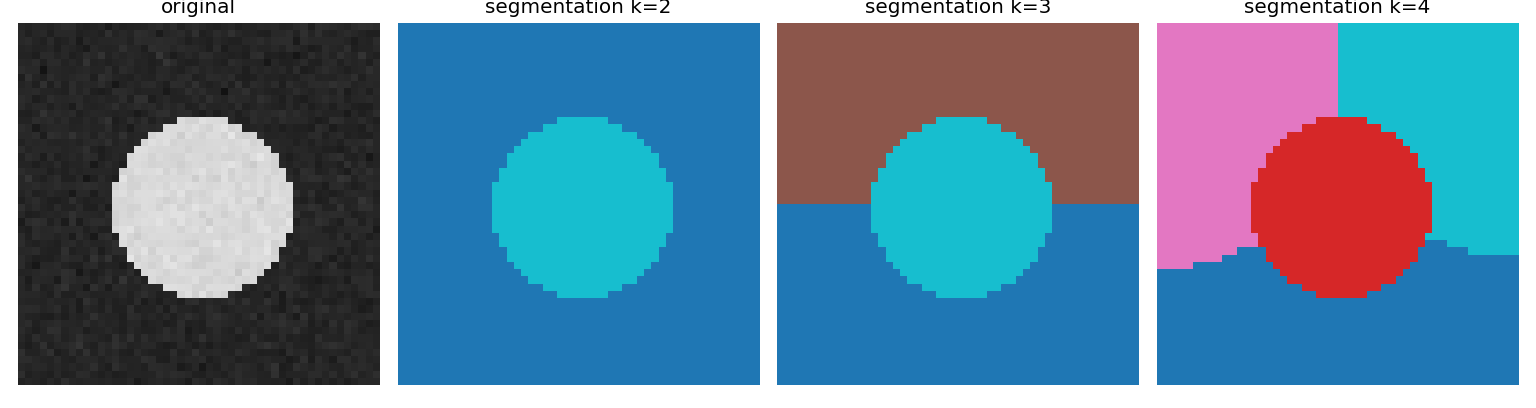
\includegraphics[width=\linewidth]{../Q4-CODE/outputs/step6_segmentation.png}\\[4pt]
{\small تصویرِ اصلی در کنارِ نتیجه‌ی قطعه‌بندی برای $k=2,3,4$.}
\end{center}

\newpage
%==================================================================
\section{پرسش ۷ --- الگوریتم لانتساش}
%==================================================================

%------------------------------------------------------------------
\subsection{ایده‌ی کلی}
%------------------------------------------------------------------

الگوریتمِ لانتساش در واقع نسخه‌ی بهینه‌شده‌ای از «الگوریتمِ آرنولدی» برای ماتریس‌های \emph{متقارن} است و بر پایه‌ی مفهومِ زیرفضای کرایلف بنا شده است. ایده‌ی اصلی این است: به‌جای اینکه مقادیر ویژه‌ی یک ماتریسِ بسیار بزرگِ $A$ با ابعادِ $n\times n$ را مستقیماً حساب کنیم، با ضرب‌های متوالیِ ماتریس در یک بردار ($v,\,Av,\,A^2v,\dots$) یک زیرفضای کوچک‌تر به نامِ فضای کرایلف $\mathcal K_m$ می‌سازیم:
\[
\mathcal{K}_m(A,v)=\operatorname{span}\{v,\,Av,\,A^2v,\dots,A^{m-1}v\}.
\]
لانتساش با استفاده از یک رابطه‌ی بازگشتیِ سه‌جمله‌ای یک پایه‌ی متعامدِ یکه برای این فضا می‌سازد. نتیجه‌ی این کار، تصویرکردنِ ماتریسِ غول‌پیکرِ $A$ روی یک ماتریسِ بسیار کوچک‌تر به نامِ $T_m$ (با ابعادِ $m\times m$) است که ساختاری \textbf{سه‌قطری} دارد. مقادیر ویژه‌ی ماتریسِ کوچکِ $T_m$ (که به آن‌ها مقادیرِ ریتز می‌گویند) تقریبِ بسیار خوبی برای مقادیر ویژه‌ی حدیِ (بزرگ‌ترین و کوچک‌ترین‌های) ماتریسِ $A$ هستند.

%------------------------------------------------------------------
\subsection{رابطه‌ی بازگشتیِ سه‌جمله‌ای}
%------------------------------------------------------------------

به‌دلیلِ تقارنِ $A$، هر بردارِ پایه‌ی جدید فقط به \emph{دو بردارِ قبلی} وابسته است؛ پس گرام--اشمیت به یک رابطه‌ی بازگشتیِ سه‌جمله‌ای ساده تبدیل می‌شود. کافی است با یک بردارِ یکه‌ی اولیه‌ی $q_1=v/\norm{v}$ شروع کنیم و در هر گام این چهار محاسبه را انجام دهیم:

\begin{enumerate}[leftmargin=1.8em,itemsep=2pt,topsep=3pt]
\item یک ضربِ ماتریس--بردار و کم‌کردنِ سهمِ بردارِ قبلی: $\;w = A q_j - \beta_{j-1}\,q_{j-1}$.
\item درایه‌ی قطرِ اصلی: $\;\alpha_j = q_j\T w$.
\item حذفِ مؤلفه‌ی $q_j$ از $w$: $\;w \leftarrow w - \alpha_j q_j$.
\item درایه‌ی کنارِ قطر و بردارِ بعدی: $\;\beta_j = \norm{w}_2$ و $\;q_{j+1} = w/\beta_j$.
\end{enumerate}

\noindent (با قراردادِ $\beta_0=0$ و $q_0=\mathbf 0$؛ در عمل گامِ ۳ را برای پایداری دوباره تکرار می‌کنیم.) با کنارِ هم گذاشتنِ بردارها به‌صورتِ ستون‌های $Q_m=[\,q_1\,\cdots\,q_m\,]$، ماتریسِ سه‌قطریِ حاصل چنین است:
\[
T_m=Q_m\T A Q_m=
\begin{pmatrix}
\alpha_1 & \beta_1 & & \\
\beta_1 & \alpha_2 & \beta_2 & \\
& \beta_2 & \ddots & \ddots\\
& & \ddots & \alpha_m
\end{pmatrix}.
\]
یعنی روی قطرِ اصلی $\alpha$-ها و روی دو قطرِ کناری $\beta$-ها می‌نشینند. چون یافتنِ مقادیر ویژه‌ی یک ماتریسِ سه‌قطری ارزان است، این مقادیر (تقریبِ خوبی از مقادیر ویژه‌ی $A$) را حساب می‌کنیم و بردارهای ویژه‌ی $A$ را هم از رابطه‌ی $x=Q_m y$ بازسازی می‌کنیم که در آن $y$ بردارِ ویژه‌ی $T_m$ است.

%------------------------------------------------------------------
\subsection{مزیت نسبت به روش‌های قبلی}
%------------------------------------------------------------------

\smallskip
\noindent$\bullet$~لانتساش به $A$ تنها از راهِ $Av$ دسترسی دارد و هیچ نیازی به
ساختن، معکوس کردن یا تجزیه‌ی $A$ ندارد. چون ماتریسِ $W$ (و در نتیجه $L_{\mathrm{sym}}$)
در مسئله‌ی ما \emph{تُنُک} است، هر ضرب تنها $O(\mathrm{nnz})$ هزینه دارد، که برای تصاویرِ
بزرگ بسیار به‌صرفه است.

\smallskip
\noindent$\bullet$~برخلافِ روشِ توانِ معکوس $+$ حذف که بردارها را
\emph{یکی‌یکی} پیدا می‌کند و خطای حذف در هر مرحله انباشته می‌شود، لانتساش چند بردارِ ویژه‌ی کرانی را
هم‌زمان و با همگراییِ سریع به دست می‌دهد.

\smallskip
\noindent$\bullet$~روشِ توانی در هر تکرار بردارِ قبلی را دور می‌اندازد و فقط با بردارِ جدید کار می‌کند؛ اما لانتساش با ساختنِ زیرفضای کرایلف اطلاعاتِ همه‌ی ضرب‌های پیشین ($v,Av,A^2v,\dots$) را نگه می‌دارد و از ترکیبِ خطیِ آن‌ها برای تقریبِ بهتر بهره می‌برد؛ به همین دلیل همگراییِ آن به‌مراتب سریع‌تر است.

\smallskip
\noindent$\bullet$~حافظه و محاسباتش با $n$ به‌صورتِ خطی (با ضریبِ $m\ll n$)
رشد می‌کند، در حالی‌که روش‌های متراکم $O(n^3)$ هستند.

\smallskip
\noindent$\bullet$~در حسابِ ممیزِ شناور، تعامدِ بردارهای $q_j$ به‌مرور از بین می‌رود و
مقادیر ویژه‌ی کاذب ظاهر می‌شوند؛ به همین دلیل از متعامدسازیِ مجدد (کامل یا گزینشی)
استفاده می‌کنیم.

\noindent چون در قطعه‌بندی به کوچک‌ترین مقادیر ویژه نیاز داریم، لانتساش را یا
روی عملگرِ شیفت‌ومعکوسِ $(\mu I-L_{\mathrm{sym}})^{-1}$ اجرا می‌کنیم یا روی $2I-L_{\mathrm{sym}}$؛
این دومی کوچک‌ترین مقادیر ویژه‌ی $L_{\mathrm{sym}}$ را به بزرگ‌ترین‌ها تبدیل می‌کند و لانتساش هم به
بزرگ‌ترین‌ها سریع همگرا می‌شود.

\begin{center}
\begin{minipage}{\linewidth}
\centering
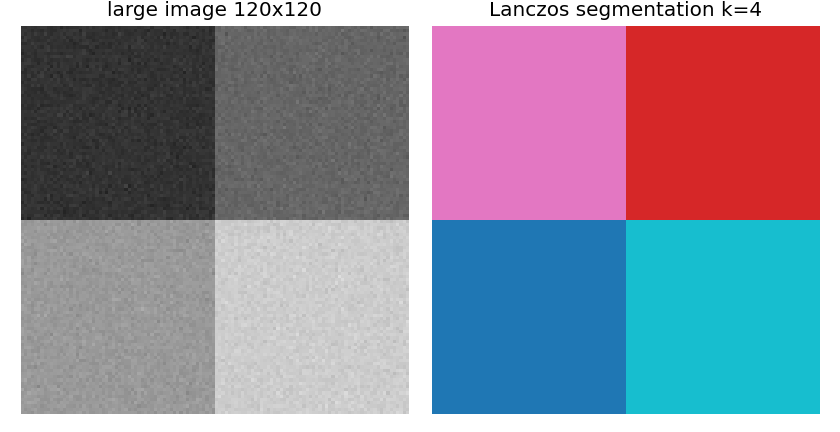
\includegraphics[width=\linewidth]{../Q4-CODE/outputs/step7_lanczos.png}\\[4pt]
{\small قطعه‌بندیِ یک تصویرِ بزرگ با لانتساش روی ماتریسِ تُنُک.}
\end{minipage}
\end{center}

\end{document}
